\chapter{Konzept, Architektur und Implementierung}
\label{ch:KonzeptArchitekturImplementierung}
Nachdem in Kapitel \ref{ch:EntwicklungDerMethodik} die Herausforderungen bei der Adaption des Ansatzes von \textcite{He_2023_ICCV} identifiziert werden, dient das vorliegende Kapitel der detaillierten Ausarbeitung der entwickelten Lösungsansätze. Wir beschreiben hier die finale Architektur und das zugrundeliegende Konzept der Online-Daten-Augmentierung. Der Fokus liegt auf der präzisen Darstellung der Methodik, von der Online-Generierung formverzerrter Bilder über den Aufbau der Netzarchitektur bis hin zur praktischen Implementierung der gesamten Pipeline.





\section{Architektur zur Online-Generierung formverzerrter Bilder}
\label{sec:ArchitekturOnlineGenerierung}

Die Qualität von Merkmalen, die für Visual Servoing eingesetzt werden, hängt entscheidend von der Robustheit des zugrundeliegenden Detektions- und Deskriptorsystems ab. Traditionelle Verfahren der Merkmalsextraktion sind oft anfällig für texturbedingte Bildartefakte und variierende Umgebungsbedingungen. Dies beeinträchtigt die Leistungsfähigkeit der visuellen Regelung. Zur Überwindung dieser Limitationen zielt diese Arbeit auf die Stärkung des \textbf{Shape-Bias} gegenüber dem \textbf{Texture-Bias} ab, inspiriert durch die Forschung von \textcite{Zhang_2023_arXiv}. Hierbei wird die Merkmalserkennung verstärkt auf die strukturelle Form von Objekten trainiert, anstatt auf feine, oft unzuverlässige Texturmerkmale.

Um dieses Ziel zu erreichen, wird ein Ansatz zur Online-Augmentierung von Bilddaten implementiert, der sich an der Architektur von \textcite{He_2023_ICCV} orientiert. Dieses Verfahren nutzt ein \textbf{\ac{GAN}}, das in der Lage ist, Bilder so zu modifizieren, dass diese eine reduzierte Textur und verstärkte sowie deformierte Kanten aufweisen. Der Fokus dieser Methode liegt auf der gezielten Manipulation von Trainingsdaten, um einen nachfolgenden Keypoint-Detektor und -Deskriptor \textendash~in diesem Fall \textbf{\ac{xFeat}} \textendash~verstärkt auf Kantenmerkmale und nicht auf Texturmerkmale zu trainieren.

\begin{figure}[htpb]
    \centering
    % Die PDF-Datei (erste Seite) wird eingebunden
    % trim = links unten rechts oben (in Punkten), clip = zuschneiden aktivieren
    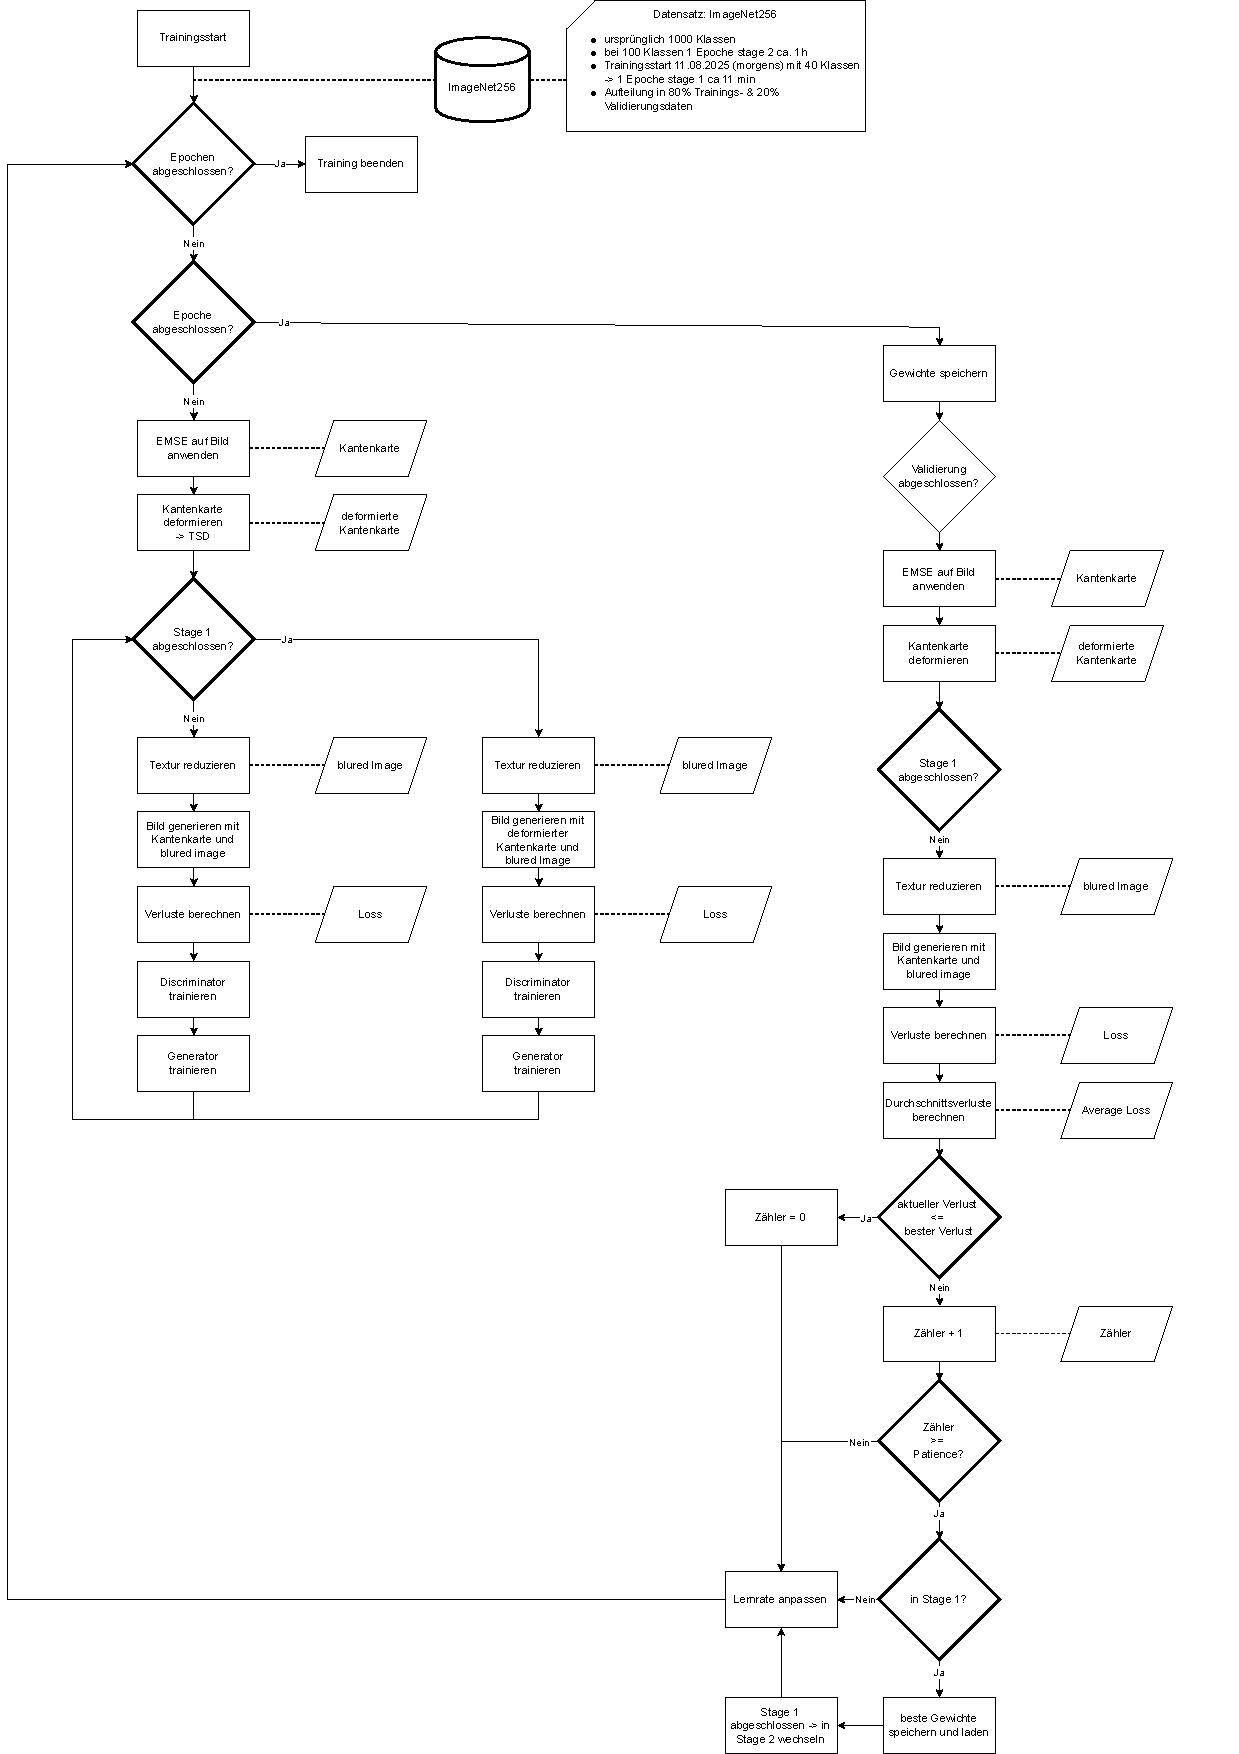
\includegraphics[clip, trim=0cm 0cm 0cm 0cm, width=\VarPicWidthB]{Figures/pdf/Ablauf_SDbOA.pdf} % trim = L B R O
    \caption{Ablauf SDbOA}
    \label{fig:Ablauf_SDbOA}
\end{figure}

\subsection{Aufbau der Online-Augmentierung}
Die Architektur zur Online-Generierung formverzerrter Bilder wird als eigenständiges Modul konzipiert und direkt in die Trainingspipeline von \ac{xFeat} integriert. Diese Integration erfolgt online, sodass die generierten Bilder in Echtzeit während des Trainings zur Verfügung stehen. Das gesamte Verfahren, schematisch dargestellt in Abbildung~\ref{fig:Ablauf_SDbOA}, basiert auf einer \textbf{zweistufigen Strategie}, die darauf abzielt, die Fähigkeit des \ac{GAN} zu optimieren, Bilder mit originalgetreuer Form, aber mit reduzierter Textur und verstärkten Kanten zu generieren.

Der Workflow beginnt mit dem Trainingsstart auf dem Datensatz ImageNet256~\cite{Uriot2023imageNet}. Die Wahl dieses Datensatzes gegenüber einem kleinskaligen Datensatz wie CIFAR-10~\cite{Uriot2023imageNet} ist von zentraler Bedeutung für die Übertragbarkeit der Ergebnisse. Bei einer Auflösung von $32 \times 32$ Pixeln ist CIFAR-10~\cite{Uriot2023imageNet} als Datensatz für die robuste Feature-Detektion und -Deskription nicht ausreichend. \ac{xFeat} benötigt eine deutlich höhere Detailgenauigkeit, die nur durch eine höhere Auflösung gewährleistet wird. Obwohl der reguläre ImageNet-Datensatz mit seinen noch höheren Auflösungen ideal wäre, stellt ImageNet256 einen strategischen Zwischenschritt dar. Die höhere Variabilität und die für \ac{xFeat} benötigte Auflösung werden bereitgestellt, während der Trainingsprozess aufgrund der reduzierten Bildgröße im Vergleich zum vollen ImageNet erheblich beschleunigt wird.

Das Training durchläuft mehrere Epochen, die jeweils als abgeschlossen markiert werden, sobald der gesamte Datensatz verarbeitet ist. Die Epoche dient als zentraler Maßstab für den Trainingsfortschritt und die Leistungsbewertung. Die Aufteilung des Trainings in zwei Phasen ermöglicht eine schrittweise Annäherung an das endgültige Ziel der robusten Merkmalsgenerierung.














\subsection{Aufbau der Online-Augmentierung}
\label{sec:Aufbau_SDbOA}
 
Die Architektur zur Online-Generierung formverzerrter Bilder ist als eigenständiges Modul konzipiert, das in die Trainingspipeline von \ac{xFeat} integriert wird. Abbildung~\ref{fig:Ablauf_SDbOA} zeigt schematisch den Ablauf des Generator-Trainings. Inspiriert von~\textcite{He_2023_ICCV} basiert das Netztraining auf einer \textbf{zweistufigen Strategie}. Dies dient dem Ziel Originalgetreue Bilder mit verstärkten Kanten sowie reduzierter Textur zu generieren.

Der Workflow beginnt mit dem \textbf{Trainingsstart} auf dem Datensatz \textbf{ImageNet256}~\cite{Uriot2023imageNet}. Das Training durchläuft mehrere Epochen, die jeweils als abgeschlossen markiert werden, sobald der gesamte Datensatz verarbeitet ist.

\newpage



\subsubsection{Phase 1: Erzeugung von Textur-reduzierten Bildern ohne Kantenverformung}
In der ersten Phase des Trainings wird keine Kantendeformierung angestrebt. Hier wird der Generator des \ac{GAN} trainiert, um ein \enquote{grob-generiertes} Bild zu erzeugen. Dies wird mit einem texturreduzierten Bild sowie der zugehörigen Kantenkarte erzeugt. Ziel ist, dass das Generator-Netz viel Information aus der Kantenkarte \enquote{nutzt} und lediglich für die korrekte Farbdarstellung auf das texturreduzierte Bild \enquote{zurückgreift}.

Die Texturreduktion des Eingangsbilds erfolgt durch ein downsampling des Originalbildes und anschließender bilinearer Interpolation~\cite{He_2023_ICCV}:
\begin{equation}
    I_{txt}=Interp(DS(I_{orig})), 
\end{equation}
wobei $I_{orig}$ als Originalbild zu verstehen ist, $DS()$ und $Interp()$ für das downsampling sowie die bilineare Interpolation und $I_{txt}$ als das texturreduzierte Bild.

Im Gegensatz zu den in~\cite{He_2023_ICCV} dargestellten Ergebnissen findet bei der Verwendung von Bildern mit einer Auflösung von $256 \times 256$ Pixeln, anstelle von $32 \times 32$ Pixeln, keine Verschiebung hin zu einem Shape-Bias statt. Ein speziell entwickeltes Diagnosetool \todo[author=Tim]{Diagnosetool beschreiben.} (siehe~\ref{??}) demonstriert, dass in mehreren Trainingsläufen mit unterschiedlich stark texturreduzierten Eingangsbildern das Modell die zur Bildgenerierung notwendigen Informationen nahezu vollständig aus den texturreduzierten Bildern extrahiert. Gleichzeitig wird die Kantenkarte weitgehend ignoriert. Dieses Verhalten belegt Abbildung~\ref{fig:Kantenverlust}. Unabhängig vom Grad der Texturreduktion hat die Kantenkarte nahezu keinen Einfluss auf den Bildgenerierungsprozess. Dies legt die Vermutung nahe, dass in der zweiten Phase des Trainings eine Deformation der Kanten vermieden wird.

\begin{figure}[htbp]
\centering
\begin{subfigure}[t]{\VarPicWidthF}
	\centering
    % trim = links unten rechts oben (in Punkten), clip = zuschneiden aktivieren
    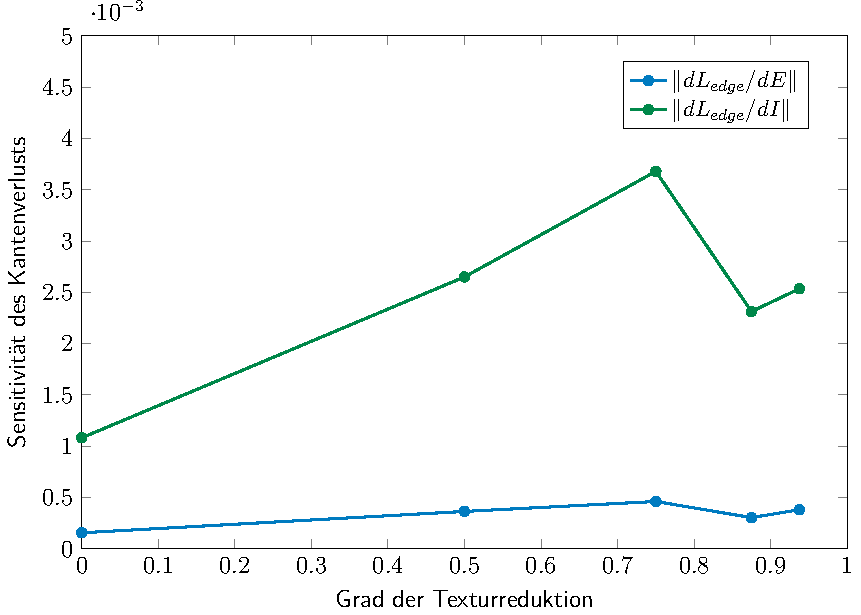
\includegraphics[clip, trim=0cm 0cm 0cm 0cm, width=\VarPicWidthA]{Figures/pdf/Ledge_vs_dsRate.pdf} % trim = L B R O
	\caption{Gradientennorm des Kantenverlusts ($L_{edge}$) in Bezug auf den Kanten-Eingang ($E$) und den Textur-Eingang ($I_{txt}$) als Funktion der Downsampling-Rate.}
	\label{fig:Sens_Kantenverlust}
\end{subfigure}
\hfill
\begin{subfigure}[t]{\VarPicWidthF}
	\centering
    % trim = links unten rechts oben (in Punkten), clip = zuschneiden aktivieren
    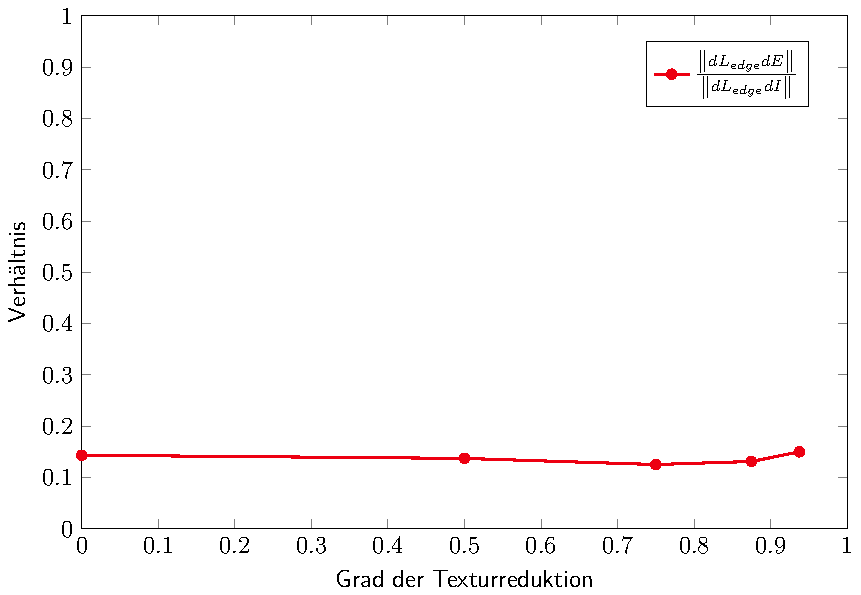
\includegraphics[clip, trim=0cm 0cm 0cm 0cm, width=\VarPicWidthA]{Figures/pdf/ratioEI_vs_dsRate.pdf} % trim = L B R O
	\caption{Verhältnis der Gradientennormen als Funktion der Downsampling-Rate. Dieser Wert visualisiert die relative Bedeutung des Kanten-Eingangs im Vergleich zum Textur-Eingang für die Generierung von Kanteninformationen.}
	\label{fig:Verhaeltnis_Sens_Kantenverlust}
\end{subfigure}
\caption{Analyse der Nutzung von Kanten- und Texturinformationen durch den Generator bei variierender Downsampling-Rate der Texturkarte.}
\label{fig:Kantenverlust}
\end{figure}

Um den Einfluss der Kantenkarte auf die Bildgenerierung zu erhöhen, respektive den Shape-Bias zu fördern, wird ein variabler Gaussian Blur auf die Eingangsbilder angewendet. Dieser Ansatz ermöglicht, die Intensität der Texturreduktion dynamisch zu steuern. Die Implementierung der Unschärfe erfolgt über eine spezielle Downsampling-Funktion, die sowohl die Stärke der Unschärfe als auch eine vollständige Texturentfernung probabilistisch steuert.

Mit einer Wahrscheinlichkeit von $p_{heavy}$ wird ein starkes Downsampling auf die geringe Größe $heavy_{down} \times heavy_{down}$ angewendet.
Andernfalls wird der Downsampling-Faktor zufällig innerhalb eines Bereichs von $[down_{min}, down_{max}]$ gewählt, wodurch eine moderate Texturreduktion erreicht wird.
Zusätzlich besteht eine Wahrscheinlichkeit von $p_{zero}$, dass das Eingangsbild vollständig mit Nullwerten gefüllt wird.
Dies entspricht einem harten Texture-Dropout.
Unabhängig von der gewählten Methode wird anschließend eine bilineare Interpolation auf die Originalgröße durchgeführt.
Optional kann dem resultierenden Bild noch leichtes Rauschen mit einer Standardabweichung von $noise_{std}$ hinzugefügt werden.
\missingfigure[figwidth=\VarPicWidthD, figheight=0.67*\VarPicWidthD]{Ggf. Variabler blur bei Eingabe netG.}

Die Generierung der Kantenkarte muss zwei kritische Anforderungen erfüllen:
\begin{enumerate}
    \item Die Kantenkarte muss differenzierbar sein, um eine korrekte Verlustrückpropagierung zu ermöglichen, und 
    \item für die gegebene Bildgröße geeignete Ergebnisse liefern.
\end{enumerate}
Die ursprüngliche \textit{\ac{EMSE}}-Methode aus~\cite{He_2023_ICCV}, die auf dem nicht-differenzierbaren Canny-Algorithmus basiert und eine ineffiziente CPU-Verarbeitung nutzt, ist für eine nahtlose Integration in eine \textbf{End-to-End}-Trainingspipeline ungeeignet. Um diese Problematiken zu beheben, wird die \textit{\ac{DS-EMSE}}-Methode eingeführt.

Die hier vorgeschlagene \textit{\ac{DS-EMSE}}-Methode überwindet diese Einschränkungen, indem eine vollständig differenzierbare Kantenextraktion implementiert wird. Anstelle des nicht-differenzierbaren Canny-Algorithmus wird der Sobel-Filter verwendet, um die Kanten zu berechnen.

Die Implementierung umfasst folgende Schritte:
\begin{enumerate}
\item Das Eingangsbild ($I_{orig}$) wird in ein Graustufenbild konvertiert, um die Komplexität zu reduzieren und sich auf Luminanzunterschiede zu konzentrieren.
\item Ein zweidimensionales Faltungsnetzwerk (PyTorch) wendet die horizontalen ($K_x$) und vertikalen ($K_y$) Sobel-Filter-Matrizen an~\cite{Sobel2014operator}. Dies ermöglicht die Berechnung der Ableitungen sowohl in horizintaler x-Richtung ($G_x$) sowie vertikaler y-Richtung ($G_y$).
\item Die Kantenstärke (Magnitude) wird als $\sqrt{G_x^2 + G_y^2}$ berechnet. Dies stellt die Aggregation der Gradienteninformationen über beide Achsen hinweg.
\item Das resultierende Kantenstärkenbild wird normalisiert und invertiert. Dies stellt sicher, dass Kanten einen geringen (schwrze Pixel) und Hintergründe einen hohen (weiße Pixel) Wert aufweisen.
\item Das einkanalige, invertierte Kantenstärkenbild wird auf drei Kanäle repliziert, um der erwarteten Eingabe des Generator-Netzes zu entsprechen.
\end{enumerate}
Im Gegensatz zur Canny-basierten \textit{\ac{EMSE}}-Methode, die eine Kantenkarte als binäres (schwarz-weißes) Bild liefert, erzeugt die \textit{\ac{DS-EMSE}}-Methode eine Kantenkarte mit Graustufen. Diese Graustufen-Kantenkarte repräsentiert die Stärke der Kanten an jeder Stelle im Bild und ermöglicht es dem Netzwerk, subtile Gradientenunterschiede zu nutzen. Dies führt zu einer höheren Informationsdichte in der Kantenkarte, was sich positiv auf das Training des Generators auswirkt. Die durchgängige Differenzierbarkeit innerhalb der PyTorch-Umgebung eliminiert die Notwendigkeit von \ac{CPU}-Transfers und ermöglicht eine nahtlose Integration in die Backpropagation.
\missingfigure[figwidth=\VarPicWidthD, figheight=0.67*\VarPicWidthD]{Evtl. Grafik EMSE vs. DS-EMSE.}

\subsubsection{Verlustfunktion und Gewichtung}
Die Verlustfunktion $L_{1st}$ in der ersten Trainingsphase dient der initialen Generierung eines grob-generierten Bildes. Die von~\textcite{He_2023_ICCV} ursprünglich definierte Verlustfunktion für die erste Phase setzt sich aus dem
\begin{itemize}
    \item dem adversarial loss ($L_{gan}$),
    \item dem $L_1$-Verlust ($L_L1$) sowie
    \item dem Cross-Entropy-Verlust ($L_{CE}$)
\end{itemize}
zusammen:
\begin{equation}
    L_{1st} = \lambda_{GAN} L_{gan} + \lambda_{L1} L_{L1} + \lambda_{cls} L_{CE}
\end{equation}

Dabei entsprechen die Terme den folgenden Komponenten:
\begin{itemize}
\item \textbf{Adversarial Loss ($L_{gan}$)}: Dieser Verlustterm ist der zentrale Bestandteil des \ac{GAN}-Trainings. Er regelt die Konkurrenz zwischen dem Generator und dem Diskriminator. Der Generator wird trainiert, um Bilder zu erzeugen, die vom Diskriminator als \enquote{real} eingestuft werden, während der Diskriminator lernt, zwischen echten und generierten Bildern zu unterscheiden. Dieser Mechanismus sorgt für die fotorealistische Qualität der generierten Bilder~\cite{He_2023_ICCV}.
\item \textbf{$L_1$-Verlust ($L_L1$)}: Dieser Term misst die absolute Differenz zwischen dem generierten Bild ($I_{gen}$) und dem ursprünglichen Bild ($I_{orig}$). Er dient als starke Einschränkung, die sicherstellt, dass die grundlegenden Farben und Texturen des Originalbildes im generierten Bild beibehalten werden. Im Gegensatz zur originalen Arbeit von~\textcite{He_2023_ICCV}, die einen feature matching loss verwendet, wird hier ein direkter $L_1$-Verlust genutzt, eine Technik, die auch in anderen bildgenerierenden Modellen, wie z. B. Pix2Pix \cite{isola2018Pix2Pix}, Anwendung findet.
\item \textbf{Cross-Entropy-Verlust ($L_{cls}$)}: Dieser Verlustterm ist entscheidend für die Korrelation zwischen der generierten Form und der Texturkategorie. Er stellt sicher, dass das generierte Bild die richtige visuelle Repräsentation für die zugehörige Klasse (z. B. ein Hund, eine Katze) hat. Dies verhindert die Generierung von Bildern mit korrekter Form, aber einer inkorrekten Texturkategorie. Die Implementierung orientiert sich am ACGAN-Ansatz \cite{odena2017ACGAN}, der Klassifizierungsinformationen nutzt, um die Generierung zu steuern.
\item \textbf{Shape-Preservation Loss ($L_{edge}$)}: Dieser Term misst die $L_1$-Norm zwischen der Kantenkarte des generierten Bildes ($E_{gen}$) und der Eingabe-Kantenkarte ($E_{in}$). Er stellt sicher, dass die Kanten des generierten Bildes denen der Eingabe-Kantenkarte ähneln. Im Unterschied zur Originalarbeit, in der dieser Verlust erst in der zweiten Phase des Trainings (fine-tuning) angewendet wird, wird er hier bereits in der ersten Phase eingeführt. Dies soll sicherstellen, dass das Netzwerk von Beginn an einen starken Fokus auf die Kanten legt und somit eine schnellere Verschiebung hin zu einem ausgeprägten Shape-Bias erfolgt.
\end{itemize}
Die $\lambda$-Koeffizienten dienen der Steuerung des Einflusses der einzelnen Terme auf den Gesamtverlust. Ihre optimale Abstimmung ist entscheidend für das Gleichgewicht zwischen der Bildqualität, der Kantenwiedergabe und der korrekten Klassenzuordnung.
\missingfigure[figwidth=\VarPicWidthD, figheight=0.67*\VarPicWidthD]{Ggf. Grafik Loss über versch. Lambdas.}

\subsubsection{Phase 2: Fine-Tuning mit Kantenverformung}
\todo{Überarbeiten! (Grafiken, etc.)}

Die zweite Phase dient dem Fine-Tuning des Generators, um die Empfindlichkeit gegenüber Kantenverformungen zu verringern und das Training zu stabilisieren.
\begin{itemize}
\item \textbf{Eingabe:} Der Generator erhält nun die verformte Kantenkarte ($E_{deform}$) und das textur-reduzierte Bild ($I_{txt}$).
\item \textbf{Verlustfunktion:} Die Verlustfunktion wird um zwei zusätzliche Terme erweitert, um die Feinabstimmung zu steuern. Die endgültige Verlustfunktion $L_{2nd}$ ist die Summe aus:
\begin{itemize}
\item \textbf{Adversarial Loss} ($L_{gan}$)
\item \textbf{Cross-Entropy Classification Loss} ($L_{cls}$), um die Korrelation zwischen Kantenkarte und Textur zu stärken.
\item \textbf{Shape-Preservation Loss} ($L_{edge}$), definiert als die $L_1$-Norm zwischen der verformten Kantenkarte ($E_{deform}$) und einer aus dem synthetisierten Bild extrahierten Kantenkarte. Dieser Term dient als weiche Einschränkung, um die generierte Form nahe an der verformten Kantenkarte zu halten.
\end{itemize}
\item \textbf{Zweck:} Durch diese gezielte Überwachung wird die Fähigkeit des Generators verbessert, plausible Bilder aus verformten Kantenkarten zu erzeugen, ohne die grundlegende Objekterkennung zu beeinträchtigen.
\end{itemize}

Die Validierung und Optimierung am Ende jeder Epoche laufen wie im Diagramm beschrieben ab: Der \textbf{Durchschnittsverlust (Average Loss)} wird mit dem besten bisherigen Verlust verglichen, um die Lernrate anzupassen und die besten Gewichte zu speichern.

Dieser multistage Ansatz stellt sicher, dass der trainierte Feature-Detektor eine verbesserte Robustheit gegenüber Beleuchtungsänderungen, Oberflächenbeschaffenheit und Skalierung aufweist, da seine Merkmalserkennung von der variablen Textur entkoppelt wird.



\newpage





\section{Aufbau Netzarchitektur}
\todo{Architektur beschreiben.}
\todo[inline]{V. a., dass Zahlen für Ausgangsgrößen der Schichten stehen.}
\begin{figure}[htpb]
    \centering
    % Die PDF-Datei (erste Seite) wird eingebunden
    % trim = links unten rechts oben (in Punkten), clip = zuschneiden aktivieren
    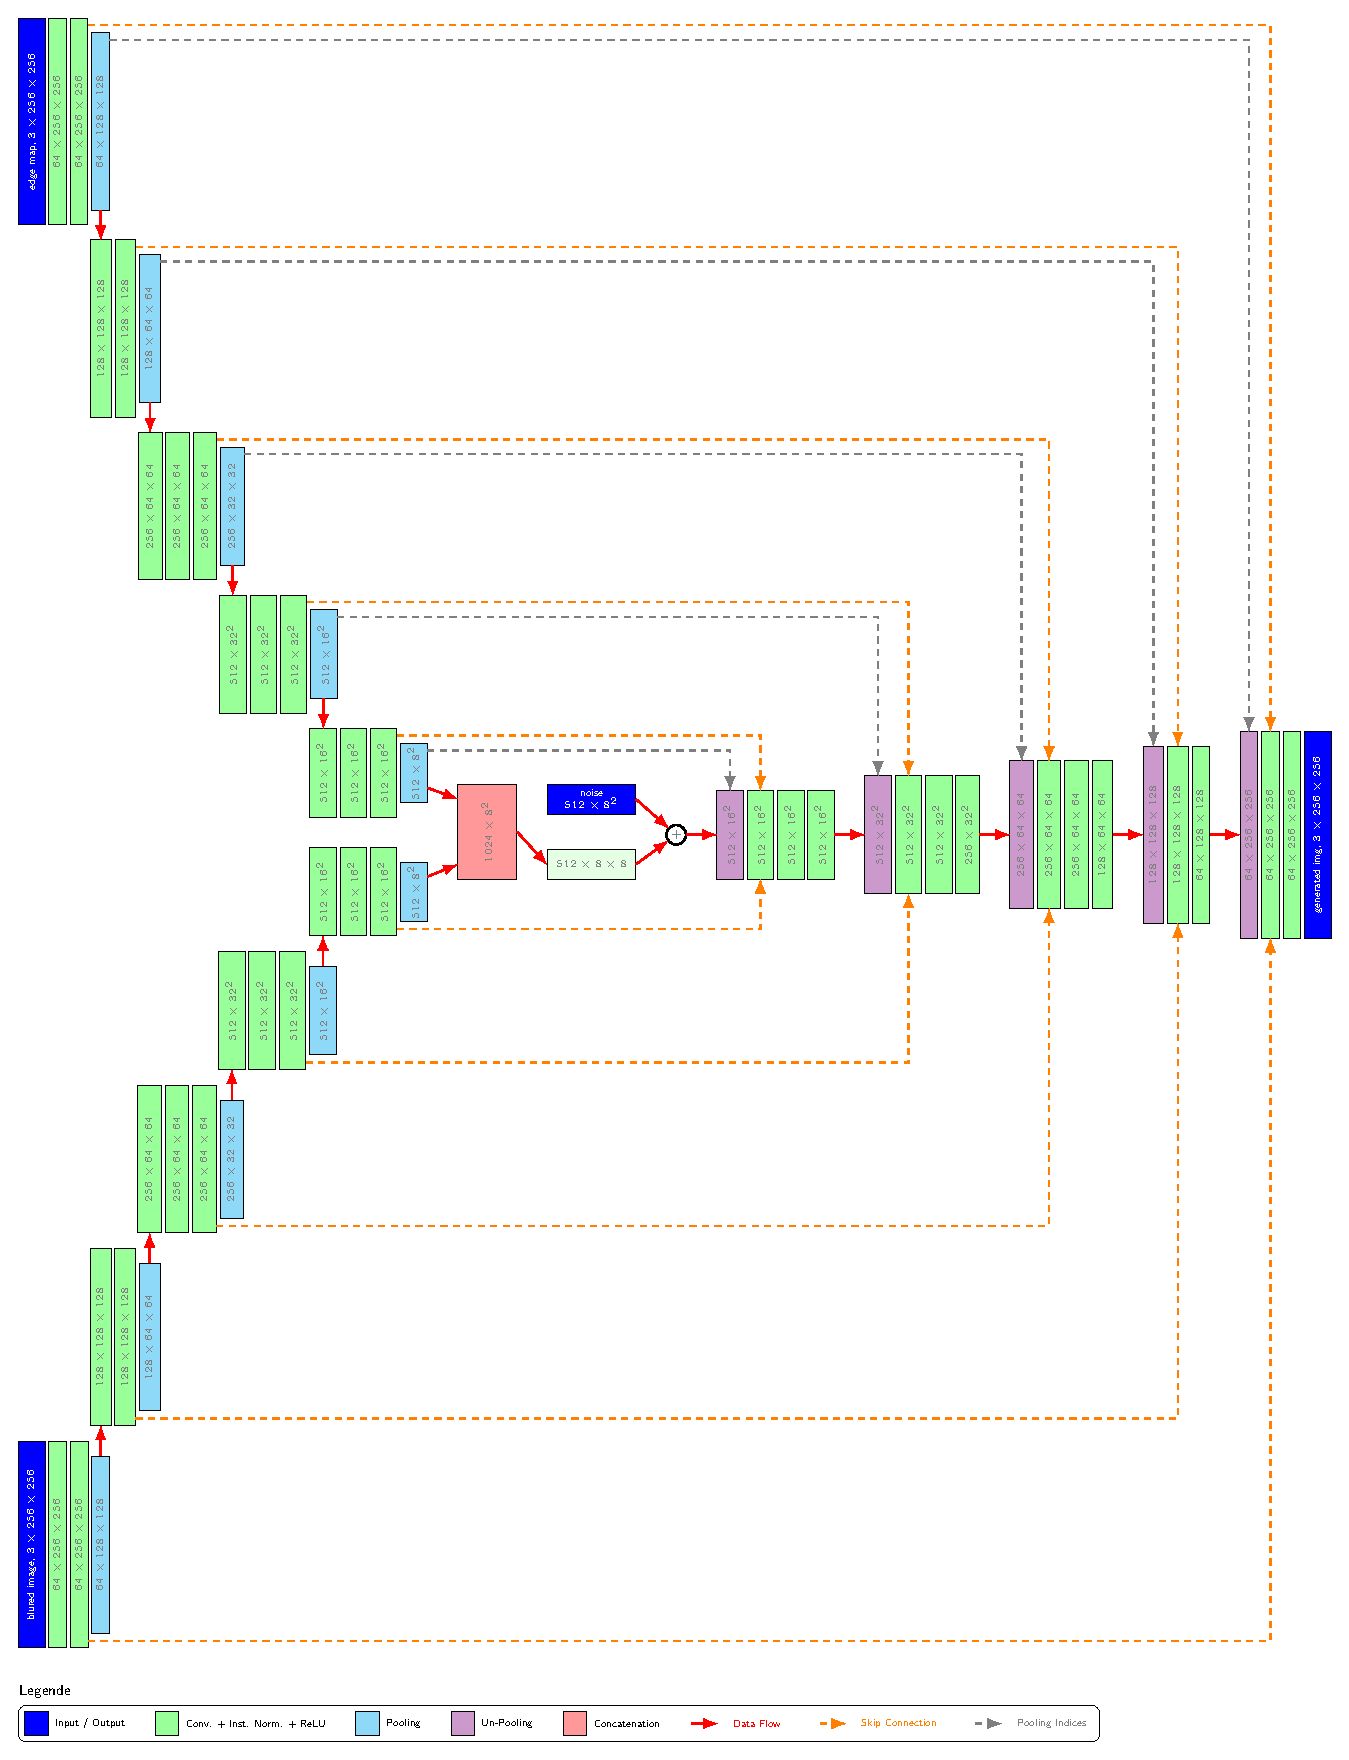
\includegraphics[clip, trim=0cm 0cm 0cm 0cm, width=\VarPicWidthB]{Figures/pdf/Generator_V2_2.pdf} % trim = L B R O
    \caption{Aufbau Netzarchitektur Generator-Netz}
    \label{fig:Aufbau_netG}
\end{figure}





\section{Kopplung von Segmentierung und Featureextraktion}
\label{sec:KopplungSegmentierungFeatureextraktion}
% TODO





\section{Implementierung der Pipeline}
\label{sec:Implementierung}
% TODO

